\section{Latency}\label{sec:latency}

The second group of experiments regards the latency and is divided into two
different analysis: the first one shows the comparison of the latency into
Dijkstra and dual ascent, considering all nodes as target. The second one,
instead, uses also non-target nodes.

\subsection{All target nodes}

This kind of experiment is done using three different topologies (in order of
size):
\begin{description}
	\item[Spine topology] A very little one, with only two spines and four
		leaves (\figref{subfig:spinetopo}).
	\item[Medium topology] Composed by 10 nodes and 20 links
		(\figref{subfig:mediumtopo}).
	\item [Paper topology] The same used for bandwidth experiments
		(\figref{fig:papertopo}).
\end{description}

\begin{figure}
	\centering
	\begin{subfigure}[b]{0.45\textwidth}
		\centering
		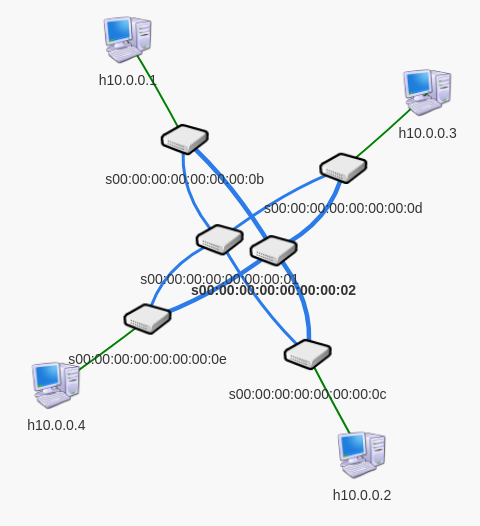
\includegraphics[width=\textwidth]{img/spinetopo.png}
		\caption{Spine topology}\label{subfig:spinetopo}
	\end{subfigure}
	\begin{subfigure}[b]{0.45\textwidth}
		\centering
		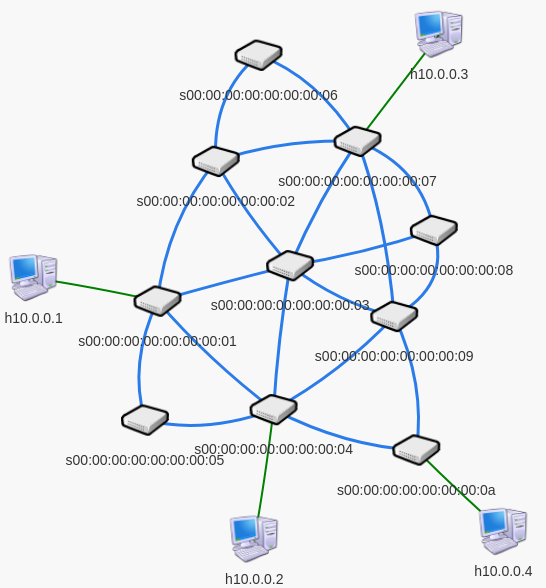
\includegraphics[width=\textwidth]{img/othertopo.png}
		\caption{Medium topology}\label{subfig:mediumtopo}
	\end{subfigure}
	\caption{Topologies used for the experiments on the costs of the two
	algorithms}\label{fig:othertopologies}
\end{figure}

For each topology we collect and compare the total costs of many executions for
both Dijkstra and dual ascent broadcast trees, finally aggregated with the
average. The results are shown in \figref{fig:avg-latency}.

\begin{figure}
	\centering
	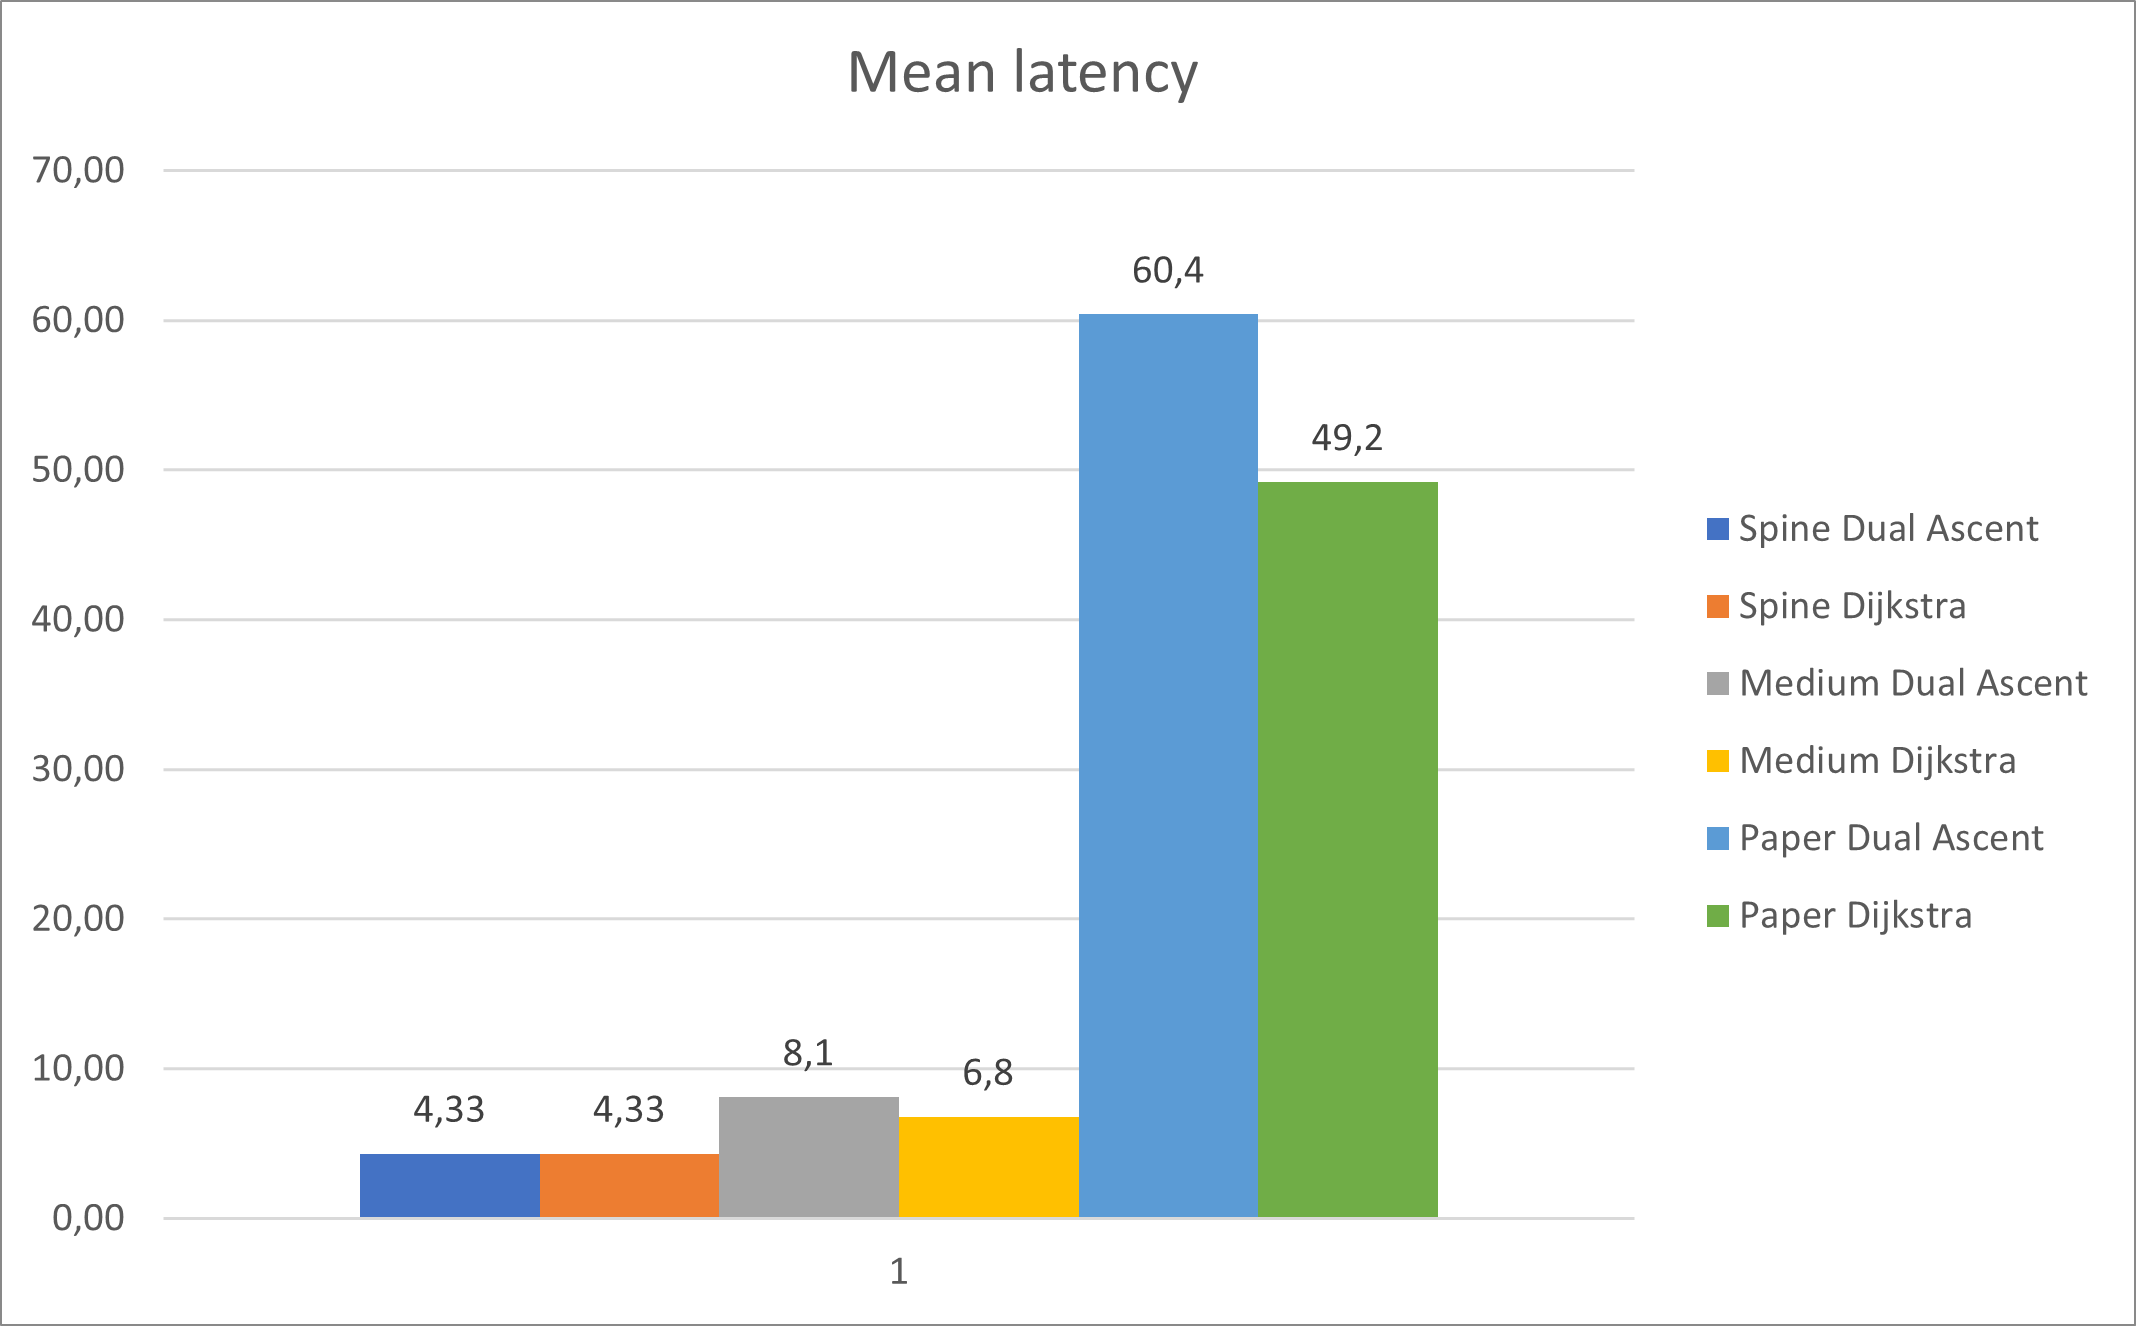
\includegraphics[width=\textwidth]{img/lat-mean-all.png}
	\caption{Latency for the three topologies using all target
	nodes}\label{fig:avg-latency}
\end{figure}

We can see that the difference from Dijkstra (always better in the analysis) and
dual ascent are minimal and grows increasing the complexity of the network, but
as in the bandwidth experiments this can't be seen as an absolute truth, because
algorithms are similar and results can depend on the Floodlight execution, so we
can have an execution or simply a different topology with minor costs for the
dual ascent setting.

\subsection{Using non-target nodes}

To see the real powerful of dual ascent we have to insert some non-target nodes
(not considered by Dijkstra). We have added a configuration, based on the paper
topology, which considers all the core nodes as non-target, so the target ones
are only the border nodes. The result target topology can be seen in
\figref{fig:paper-target}.

\begin{figure}
	\centering
	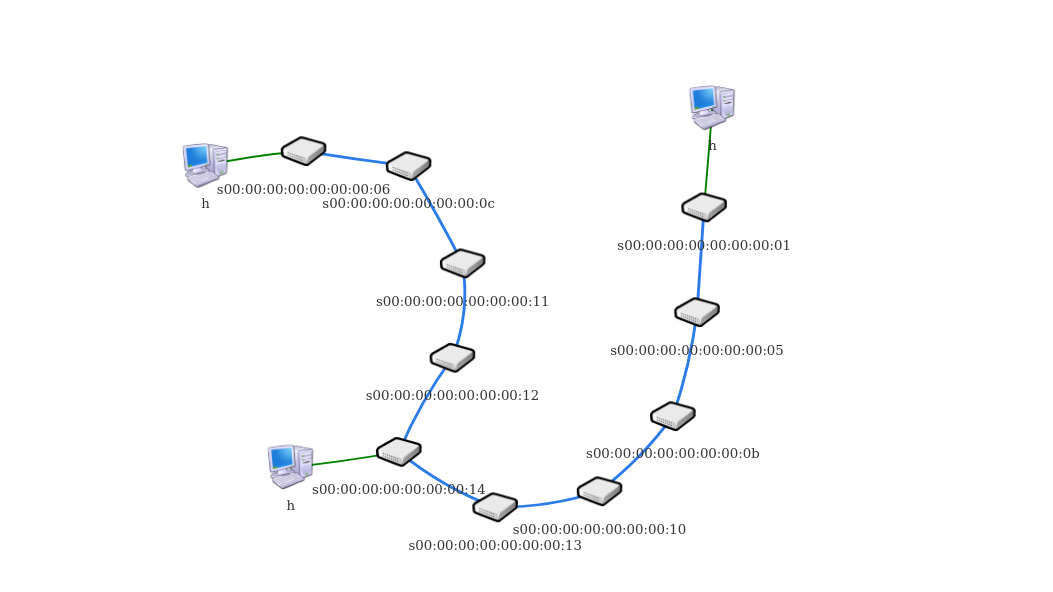
\includegraphics[width=\textwidth]{img/paper-topo-onlytarget.png}
	\caption{Paper topology considering only target
	nodes}\label{fig:paper-target}
\end{figure}

For this kind of experiments the number of hosts in the paper topology is three
instead of four. We consider the latency for the host-to-host paths and not for
the whole broadcast tree. The results are shown in
\figref{fig:lat-mean-target}.

\begin{figure}
	\centering
	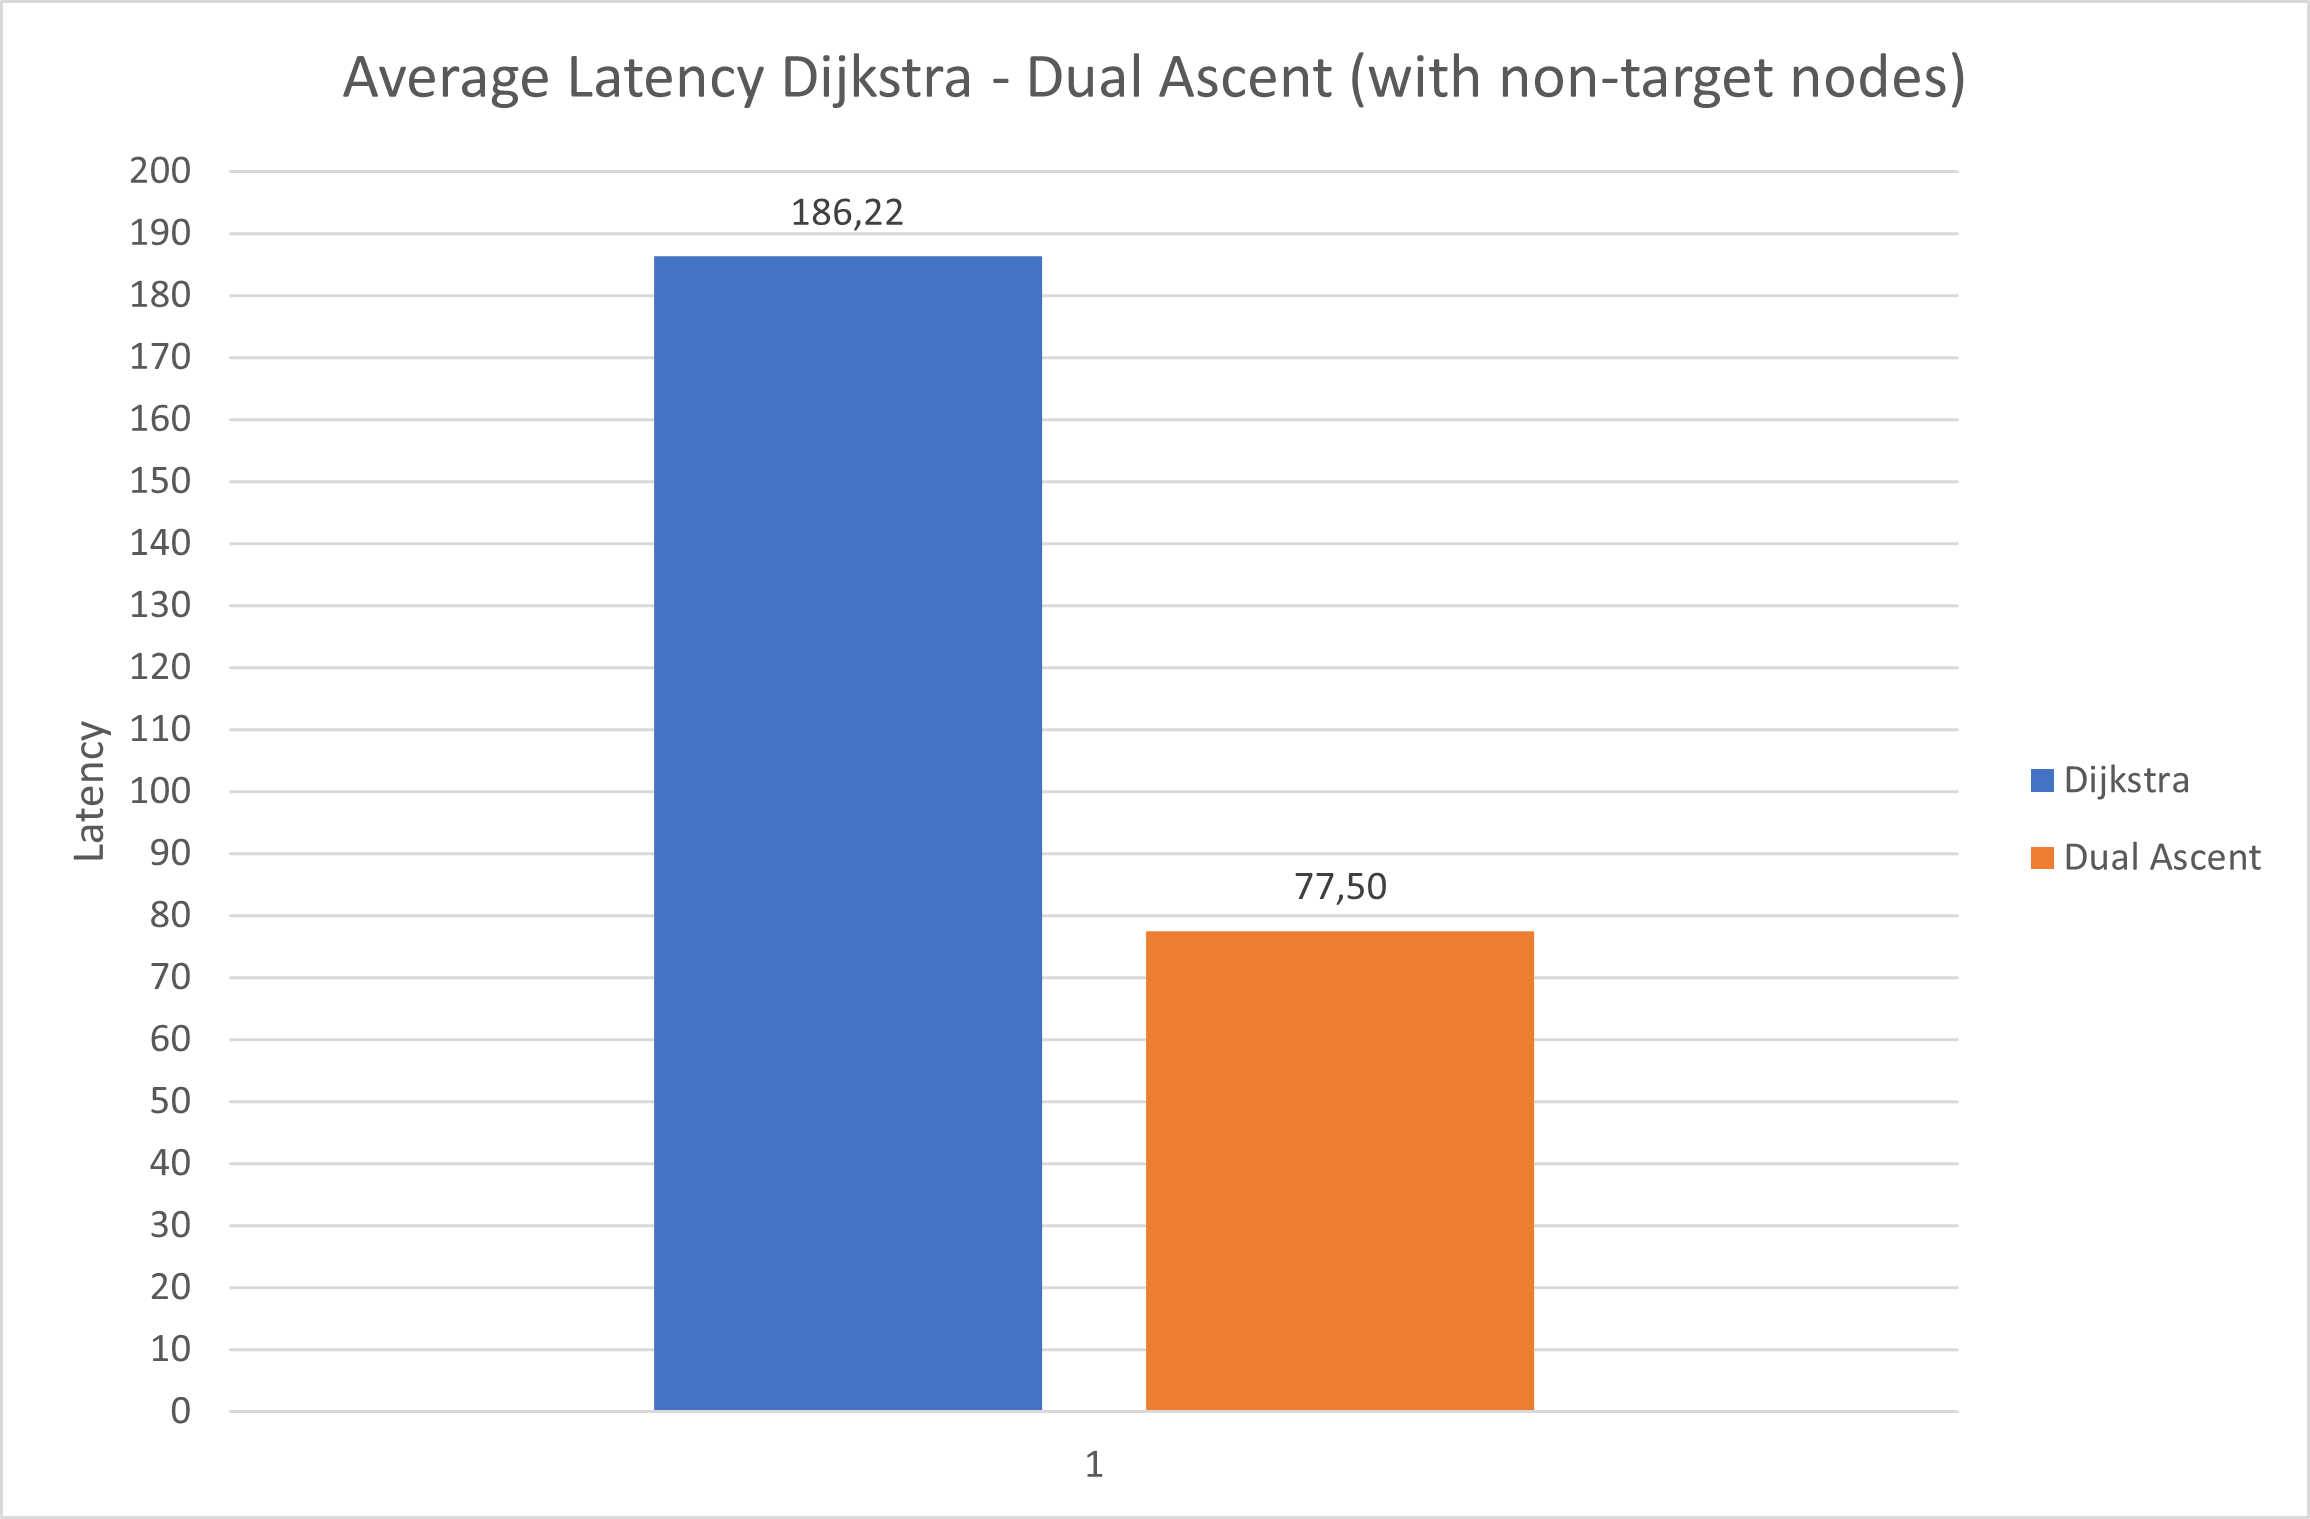
\includegraphics[width=\textwidth]{img/lat-mean-target.png}
	\caption{Latency considering some non-target
	nodes}\label{fig:lat-mean-target}
\end{figure}

As we can see in this example Dijkstra can only pass from all border nodes, so
the costs are very high with respect to dual ascent, which computes his best
path considering all the nodes to compute a broadcast tree that contains at
least all the target (border) nodes.
